%%%%%%%%%%%%%%%%%%%%%%%%%%%%%%%%%%%%%%%%%
% Jacobs Landscape Poster
% LaTeX Template
% Version 1.0 (29/03/13)
%
% Created by:
% Computational Physics and Biophysics Group, Jacobs University
% https://teamwork.jacobs-university.de:8443/confluence/display/CoPandBiG/LaTeX+Poster
% 
% Further modified by:
% Nathaniel Johnston (nathaniel@njohnston.ca)
%
% This template has been downloaded from:
% http://www.LaTeXTemplates.com
%
% 
% Masaryk University presentation themes were downloaded from:
% https://www.overleaf.com/gallery/tagged/muni
%
% and ported into Jacobs Landscape Poster by:
% Jumaidil Awal (ideal1st.here@googlemail.com)
% 
% Jacobs Landscape Poster License:
% CC BY-NC-SA 3.0 (http://creativecommons.org/licenses/by-nc-sa/3.0/)
%
% Masaryk University's fibeamer theme license:
% Copyright 2015  Vít Novotný <witiko@mail.muni.cz>
% Faculty of Informatics, Masaryk University (Brno, Czech Republic)
% under Latex Project Public License
%
%%%%%%%%%%%%%%%%%%%%%%%%%%%%%%%%%%%%%%%%%

%----------------------------------------------------------------------------------------
%	PACKAGES AND OTHER DOCUMENT CONFIGURATIONS
%----------------------------------------------------------------------------------------

\documentclass[final]{beamer}

\usepackage[scale=0.849]{beamerposter} % Use the beamerposter package for laying out the poster

%\usetheme{confposter} % Use the confposter theme supplied with this template
\usetheme[faculty=chemo]{fibeamer} % Uncomment to use Masaryk University's fibeamer theme instead.

%\setbeamercolor{block title}{fg=ngreen,bg=white} % Colors of the block titles
%\setbeamercolor{block body}{fg=black,bg=white} % Colors of the body of blocks
%\setbeamercolor{block alerted title}{fg=white,bg=ngreen} % Colors of the highlighted block titles
%\setbeamercolor{block alerted body}{fg=black,bg=dblue!10} % Colors of the body of highlighted blocks
% Many more colors are available for use in beamerthemeconfposter.sty

%-----------------------------------------------------------
% Define the column widths and overall poster size
% To set effective sepwid, onecolwid and twocolwid values, first choose how many columns you want and how much separation you want between columns
% In this template, the separation width chosen is 0.024 of the paper width and a 4-column layout
% onecolwid should therefore be (1-(# of columns+1)*sepwid)/# of columns e.g. (1-(4+1)*0.024)/4 = 0.22
% Set twocolwid to be (2*onecolwid)+sepwid = 0.464
% Set threecolwid to be (3*onecolwid)+2*sepwid = 0.708

\newlength{\sepwid}
\newlength{\onecolwid}
\newlength{\twocolwid}
\newlength{\threecolwid}
\setlength{\paperwidth}{46.8in} % A0 width: 46.8in
\setlength{\paperheight}{33.1in} % A0 height: 33.1in
\setlength{\sepwid}{0.007\paperwidth} % Separation width (white space) between columns
\setlength{\onecolwid}{0.31\paperwidth} % Width of one column
\setlength{\twocolwid}{0.451\paperwidth} % Width of two columns
\setlength{\threecolwid}{0.64\paperwidth} % Width of three columns
%\setlength{\topmargin}{-0.5in} % Reduce the top margin size
%-----------------------------------------------------------

% Theorems
\newtheorem{thm}{Theorem}[section]
%\newtheorem{proof}[thm]{Proof}
%\newtheorem{lemma}[thm]{Lemma}
\newtheorem{rem}[thm]{Remark}
\newtheorem{cor}[thm]{Corollary}
\newtheorem{ex}[thm]{Example}
\newtheorem{assu}[thm]{Assumption}
\newtheorem{alg}[thm]{Algorithm}
\newtheorem{defn}[thm]{Definition}
\newtheorem{app1}[thm]{Image Processing}
\newtheorem{app2}[thm]{Text Mining}


\usepackage{caption}
\captionsetup[figure]{labelformat=simple}

\usepackage{mathtools}
\DeclarePairedDelimiterX{\norm}[1]{\lVert}{\rVert}{#1}

\usepackage{graphicx}  % Required for including images

\usepackage{booktabs} % Top and bottom rules for tables

%----------------------------------------------------------------------------------------
%	TITLE SECTION 
%----------------------------------------------------------------------------------------

\title{The Why and How of Nonnegative Matrix Factorization} % Poster title

\author{Group 2} % Author(s)

\institute{École Polytechnique de Louvain, UCLouvain} % Institution(s)

%----------------------------------------------------------------------------------------

\begin{document}
\addtobeamertemplate{block end}{}{\vspace*{2ex}} % White space under blocks
\addtobeamertemplate{block example end}{}{\vspace*{2ex}} % White space under example blocks
\addtobeamertemplate{block alerted end}{}{\vspace*{2ex}} % White space under highlighted (alert) blocks

\setlength{\belowcaptionskip}{2ex} % White space under figures
\setlength\belowdisplayshortskip{2ex} % White space under equations
%\begin{darkframes} % Uncomment for dark theme, don't forget to \end{darkframes}
\begin{frame} % The whole poster is enclosed in one beamer frame

%==========================Begin Head===============================

  \begin{columns}[t]
   \begin{column}{\linewidth}
    \vskip0.5cm
    \centering
    \usebeamercolor{title in headline}{\color{fg}\Huge{\textbf{\inserttitle}}\\[0.3ex]}
    \usebeamercolor{author in headline}{\color{fg}\large{\insertauthor}\\[0.3ex]}
    %\usebeamercolor{institute in headline}{\color{fg}\large{\insertinstitute}\\[1ex]}
   \end{column}
  \end{columns}
 \vspace{2cm}

%==========================End Head===============================

\begin{columns}[t] % The whole poster consists of three major columns, the second of which is split into two columns twice - the [t] option aligns each column's content to the top
\begin{column}{\sepwid}
\end{column} % Empty spacer column
\begin{column}{\threecolwid}

%----------------------------------------------------------------------------------------
%	Introduction and Motivation
%----------------------------------------------------------------------------------------

\begin{exampleblock}{In a few words}
NMF is a powerful tool for the analysis of \textbf{high-dimensional} data as it automatically extracts \textbf{sparse} and \textbf{meaningful} features from a set of \textbf{nonnegative} vectors.
NMF was introduced by Paatero and Tapper %TODO bibli
in 1994 and further developped by Lee and Seung %TODO bibli
in 1999.
\end{exampleblock}

%----------------------------------------------------------------------------------------
%	Nonnegative Matrix Factorization: definition and properties (sparse, meaningful features)
%----------------------------------------------------------------------------------------

\begin{exampleblock}{Nonnegative Matrix Factorization : definition and properties}
Nonnegative matrix factorization (NMF) is a Linear dimensionality reduction (LDR). As a reminder, a LDR computes a set of $r < min(p,n)$ basis elements $w_k \in R^p$ for $1 \leq k \leq r$ to approximate a set of data points $x_j \in R^{p}$ for $1 \leq j \leq n$ such that $\forall j, x_j \approx \sum_{k = 1}^{r} w_{k} h_{j}(k)$, for some weights $h_j\in R^r$. \\
LDR is equivalent to low-rank matrix approximation where: $X \approx W H$ where \\
     \begin{itemize}
     \item $X \in R^{p \times n}$ : $X(:,j) = x_j$ for $1 \leq j \leq n$. Each column of the matrix $X$ is a data point.
     \item $W \in R^{p \times r}$ : $W(:,k) = w_k$ for $1 \leq k \leq r$. Each column of the matrix $W$ is a basis element.
     \item $H \in R^{r \times n}$ : $H(:,j) = h_j$ for $1 \leq j \leq n$. Each column of the matrix H gives the coordinates of a data point X(:,j) in the basis W.
     \end{itemize}

     \textbf{NMF} : decomposing a given nonnegative data matrix $X$ as $X \approx W H$ where $W \geq 0$ and $H \geq 0$. $W$ and $H$ are thus component-wise nonnegative.
     
\end{exampleblock}



%----------------------------------------------------------------------------------------
%	Applications
%----------------------------------------------------------------------------------------

\begin{exampleblock}{Applications}
\begin{columns}[t]
\begin{column}{\onecolwid}
\begin{block}{Image processing}
\textbf{Goal}: facial feature extraction\\
The \textbf{data matrix} $X\in\real^{p\times n}_+$ carries information about $n$ face images. Each image has $q$ pixels and therefore each column of $X$ represents an image of a face.\\
$\rightarrow$ The $(i,j)$th entry of $X$ represents the gray-level of the $i$th pixel in the $j$th face.\\
The \textbf{nonnegative matrix factorization} can be interpreted as follows:\\
\begin{itemize}
    \item Each column of the matrix $W$ represents a facial feature
    \item The $(k,j)$th entry of $H$ represents the importance of the $k$th feature in the $j$th face
\end{itemize}
\begin{figure}
    \centering
    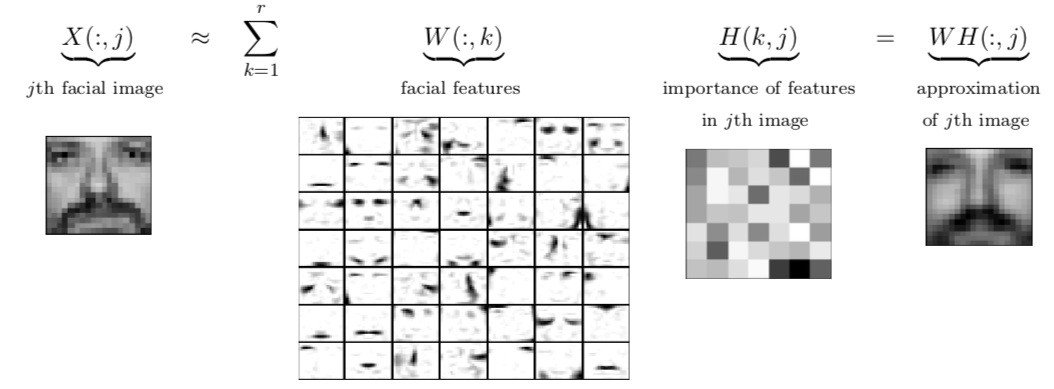
\includegraphics{../images/NMF_app1.png}
\end{figure}
\end{block}
\end{column}
\begin{column}{\onecolwid}
\begin{block}{Text Mining}
\textbf{Goal}: topic recovery and document classification\\
The \textbf{data matrix} $X\in\real^{n\times n}_+$ encodes the frequency of some words in a list of documents.\\
$\rightarrow$ The $(i,j)$th entry of $X$ represents the number of times the $i$th word appears in the $j$th document.\\
The \textbf{nonnegative matrix factorization} can be interpreted as follows:\\
\begin{itemize}
    \item Each colum of the matrix $W$ represents a topic
    \item The $(k,j)$th entry of $H$ represents the importance of the $k$th topic in the $j$th document
\end{itemize}
\begin{figure}
    \centering
    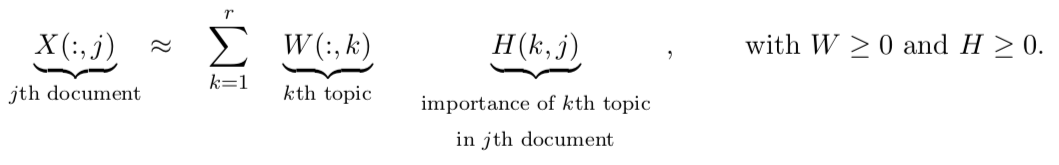
\includegraphics{../images/NMF_app2.png}
\end{figure}
\end{block}
\end{column}
\end{columns}
\end{exampleblock}

\begin{exampleblock}{Algorithms and Difficulties}
\begin{columns}[t]
\begin{column}{\onecolwid}
\begin{block}{Optimization Problem}
We want to solve \(\displaystyle \min_{W \in \mathbb{R}^{p \times r}, H \in \mathbb{R}^{r \times n}} \norm{X - WH}^2_{\textnormal{F}}\), such that \(W \geqslant 0\), \(H \geqslant 0\).
Our use of the Frobenius norm implies the assumption that the noise is Gaussian.
This is not always the best choice; in practice, depending on the application, other choices are possible too, such as:
\begin{itemize}
    \item Kullback--Leibler divergence used in text mining;
    \item Itakura--Saito distance used in music analysis;
    \item \(\ell_1\) norm used to improve robustness against outliers;
    \item etc.
\end{itemize}
\end{block}
\end{column}
\begin{column}{\onecolwid}
\begin{block}{Difficulties}
NMF is not a trivial task:
\begin{itemize}
    \item NMF is \textbf{NP-hard} because of the nonnegativity constraints.
    In the unconstrained case, SVD can be used.
    In practice, assumptions and heuristics allow us to solve the problem fairly efficiently.
    \item NMF is \textbf{ill-posed}: if \((W, H)\) is an NMF of \(X\), then so is \((W', H') = (WQ, Q^{-1}H)\), where \(WQ \geqslant 0\), \(Q^{-1}H \geqslant 0\).
    This can be solved by
    \begin{itemize}
        \item using \textbf{priors} for \(W\) and \(H\), such as sparsity;
        \item adding \textbf{regularization} terms.
    \end{itemize}
    Finding application-specific solutions is an active area of research.
\end{itemize}
\end{block}
\end{column}
\end{columns}
\end{exampleblock}

\end{column}
\begin{column}{\sepwid}
\end{column} % Empty spacer column
\begin{column}{\onecolwid} % The third column


%----------------------------------------------------------------------------------------
%	Links to other problems
%----------------------------------------------------------------------------------------

\begin{exampleblock}{Connections to other problems}
\footnotesize
In this section, we will present several connections between the NMF and other mathematical problems. But first, let us introduce the nonnegative rank.
\begin{defn}[Nonnegative rank]
Given $X \in \mathbb{R}_+^{p\times n}$, the nonnegative rank of X, denoted $\text{rank}_+(X)$ is the minimum $r$ s.t. $\exists W \in \mathbb{R}_+^{p\times r}, H \in \mathbb{R}_+^{r\times n} \text{ with } X = WH$.
\end{defn}

Intuitively, the columns of X can be seen as vectors that we want to generate from a basis formed by the columns of W. We want our basis to have as few vectors as possible.
~\\
~\\
\begin{block}{Graph theory : Bipartite dimension}
finding the bipartite dimension of a graph gives a lower bound for the nonnegative rank. Indeed, let $G(X) = (V_1 \cup V_2, E)$ be a bipartite graph induced by X (i.e. $(i,j)\in E \Leftrightarrow X_{ij}\neq 0$). 
    
    The \textbf{bipartite dimension} (or the minimum biclique cover) bc$(G(X))$ is the minimum number of bicliques needed to cover all edges in E.
    
    The rectangle covering bound : 
    \[\text{bc}(G(X))\leq \text{rank}_+(X)
\]
\end{block}
\begin{block}{Communication complexity}
We talk about communication complexity when Alice knows only $x \in \{0,1\}^m$, Bob knows only $y \in \{0,1\}^n$ and both want to compute a common function
    \[f:\{0,1\}^m \times \{0,1\}^n \rightarrow \{0,1\} : (x,y) \rightarrow f(x,y)
    \]
    While minimizing their number of bits exchanged (i.e. communication complexity).

    For the nondeterministic communication complexity of $f$ (NCC), it is also the minimum number of communications required but Alice and Bob receive a message (oracle) before they start communicating.

    We define the communication matrix $X \in \{0,1\}^{2^n\times 2^m}$ as a matrix containing the values of the function $f$ for all possible combinations of inputs.
    
    We, then, obtain a higher bound on the NCC of $f$
    \[\text{NCC of } f \leq \log_2(\text{rank}_+(X))
    \]
\end{block}

\begin{block}{Linear Optimization : Extended Formulation}
The extended formulation of a polytope P is a higher dimensional polytope Q and a linear projection $\pi$ s.t. $\pi(Q) = P$.
    \begin{align*}
    \text{(LP) } & \max & c^T x\\
     &s.t. & Ax\leq b\\
     & & x \in \mathbb{R}^n \geq 0
    \end{align*}
    Finding the minimum size of an extended formulation of the polytope defined by the constrains amounts to calculating the nonnegative rank of the slack matrix $X(i,j) = b_i-A_iv_j$. With $v_j$, the $j^{th}$ vertex of P and $\{x\in \mathbb{R}^n | b_i-A_ix\geq 0\}$ its $i^{th}$ facet.
    The reason why it is interesting to find an extended formulation is that it allows to solve the (LP) in polynomial time.
\end{block}
\begin{block}{Computational Geometry : Nested polytopes}
 In computational geometry, the nested polytopes problem is closely linked to the nonnegative rank.
\end{block}

\end{exampleblock}

%-------------------------------------------------
% CONCLUSION
%-------------------------------------------------

\begin{alertblock}{Conclusion}

To sum up, we have seen that the NMF does not only generate meaningful features, but also has many applications in various domains. Indeed, we can use nonnegative matrices to describe very different things, from pixel values, to word counts, graphs, linear optimization problems, but we can also find them in probability theory, communication complexity and many more. Although there are theoretical difficulties we have to deal with in this linear dimensionality reduction technique, such as its NP-hardness and ill-posedness, there still exist different ways to deal with them.

\end{alertblock}


%----------------------------------------------------------------------------------------
%	References
%----------------------------------------------------------------------------------------
\begin{alertblock}{References}

\begin{thebibliography}{99}
\end{thebibliography}

\end{alertblock}
\end{column}
\begin{column}{\sepwid}
\end{column} % Empty spacer column
\end{columns} % End of all the columns in the poster
\end{frame} % End of the enclosing frame
%\end{darkframes} % Uncomment for dark theme
\end{document}
